\chapter{Literature}\label{chapter:literature}

This chapter presents a systematic review of the literature on collaborative augmented reality (AR) applications in industrial settings. In contrast to more hypothesis-driven research, the systematic review process for this thesis was more exploratory. While still adhering to PRISMA, there was no pre-defined outcome. Instead, the primary intention was getting an overview of the field, identifying related work, and understanding the current state of the art. The rapid advancement of AR technologies and their increasing adoption in industrial contexts necessitates a comprehensive understanding of the current state of research, implementation challenges, and design approaches for collaborative AR systems. While previous reviews have examined AR in industrial applications \cite{deSouza2020surveyIndustrialAR} and AR-based collaboration in general \cite{Lukosch2015Collaboration}, a focused synthesis of shared-space human-human collaborative AR within industrial contexts remains limited. Unlike traditional AR applications that primarily support individual users, collaborative human-human AR systems must address complex socio-technical factors including coordination mechanisms, shared awareness, communication patterns, and multi-user interaction paradigms \cite{feng2023comprehensive}. Understanding how these systems have been designed, implemented, and evaluated in industrial contexts is crucial for advancing both theoretical knowledge and practical applications.

As a result, this systematic literature review addresses three primary research questions that collectively examine the landscape of shared-space collaborative human-human AR in industrial applications:

\begin{enumerate}
    \item \textbf{RQ1:} What types of AR collaboration have been implemented in industrial applications, and how can these be classified based on their characteristics and use cases?
    \item \textbf{RQ2:} What user experience (UX) design approaches have been utilised in collaborative augmented reality (AR) applications in industrial settings, and what evidence exists regarding their effectiveness in enhancing collaboration and user satisfaction?
    \item \textbf{RQ3:} What technical challenges have been reported in the development and implementation of collaborative augmented reality (AR) systems in industrial applications, and what solutions have been proposed to address these challenges?
\end{enumerate}

These research questions were formulated to provide a comprehensive understanding of the field while addressing both technical and human factors considerations. RQ1 seeks to establish a taxonomy of collaborative AR applications, providing a foundation for understanding the diversity of implementations. RQ2 examines the human-centred aspects of collaborative AR design, addressing user experience and effectiveness measures. RQ3 focuses on the technical infrastructure and engineering challenges, which are critical for system designers and developers. Note that the focus here is deliberately on the broader field of "AR Collaboration in industrial contexts" rather than the more specific "human-human AR collaboration in industrial contexts" as specified in the overarching RQ1 in chapter~\ref{chapter:introduction}. This is an intentional choice to broaden the scope of the review to include a wider range of applications and use cases, as well as to provide a more comprehensive understanding of the field.


\section{Methodology}
\label{sec:lit-methodology}

This systematic literature review was conducted following the Preferred Reporting Items for Systematic Reviews and Meta-Analyses (PRISMA) 2020 guidelines \cite{page2021prisma}. The PRISMA framework provides a standardised approach for conducting and reporting systematic reviews, ensuring transparency, reproducibility, and methodological rigour.

\subsection{Search Strategy}
\label{subsec:search-strategy}

The literature search was designed to comprehensively identify studies examining collaborative AR applications in industrial settings. A systematic search strategy was developed using a combination of controlled vocabulary terms and free-text keywords across multiple databases.

\subsubsection{Databases and Search Terms}

The IEEE Xplore Digital Library\footnote{\url{https://ieeexplore.ieee.org/}}, ACM Digital Library\footnote{\url{https://dl.acm.org/}}, and Elsevier Scopus\footnote{\url{https://www.scopus.com/}} were searched in order to cover core venues for human-computer interaction, computer-supported cooperative work, and industrial engineering research. All searches were executed on November 4th, 2024.

While the precise syntax was adapted to each interface, the conceptual query structure was held constant across databases. The search string comprises four keyword blocks (Blocks~A-D) that directly map onto the constructs expressed in RQ1-RQ3, plus two global limiters (publication year and language):

\begin{itemize}
    \item \textbf{Block~A - AR technology:} terms capturing augmented/mixed/extended reality hardware and software (, e.\,g., \emph{"augmented reality", "mixed reality", "smart glasses", "head-mounted display"}).
    \item \textbf{Block~B - Collaboration:} synonyms for multi-user, co-located, or remote cooperation (, e.\,g., \emph{collaborat*, cooperat*, shared experience, multi-user, remote assistance}).
    \item \textbf{Block~C - Industrial context:} vocabulary anchoring the setting to manufacturing, maintenance, or shop-floor scenarios (, e.\,g., \emph{industr*, factory, assembly line, logistics, process industry}).
    \item \textbf{Block~D - Domain exclusions:} keywords for sectors in which AR is common but not relevant to our focus, applied with a \texttt{NOT} operator (, e.\,g., \emph{gaming, tourism, medical, retail}).
    \item \textbf{Limiters:} (i) publication year \textgreater{}~2016 to reflect the era of modern AR hardware and (ii) English-language publications. The language filter could only be enforced in Scopus; hits from IEEE and ACM were screened manually for language during the eligibility check.
\end{itemize}

Table~\ref{tab:search-blocks} summarises the conceptual blocks and provides representative keywords. The full, database-specific strategies are reproduced verbatim in Appendix~\ref{appendix:search-strings} to satisfy PRISMA reporting requirements.

\begin{table}[t!]
    \centering
    \caption{Conceptual search strategy blocks. The keywords shown are illustrative; see Appendix~\ref{appendix:search-strings} for the complete lists.}
    \label{tab:search-blocks}
    \begin{tabular}{@{}p{1.2cm}p{3cm}p{7.3cm}@{}}
        \toprule
        \textbf{Block} & \textbf{Concept} & \textbf{Representative keywords} \\ \midrule
        A & AR technology & augmented reality, mixed reality, extended reality, spatial computing, head-mounted display, smart glasses \\
        B & Collaboration & collaborat*, cooperat*, shared experience, multi-user, peer-to-peer, teamwork, remote assistance \\
        C & Industrial context & industr*, manufacturing, factory, production, assembly line, maintenance, logistics, shop floor \\
        D & Domain exclusions & gaming, entertainment, tourism, medical, healthcare, retail, marketing, sports \\ \bottomrule
    \end{tabular}
\end{table}

A pseudo-code representation of the master query is provided below for clarity; angle brackets \textlangle{}\,\textrangle{} denote replacement with database-specific field tags (, e.\,g., \texttt{TITLE-ABS-KEY} in Scopus or \texttt{"All Metadata":} in IEEE Xplore):

\begin{verbatim}
<field>(Block A) AND <field>(Block B) AND <field>(Block C)
AND NOT <field>(Block D)
AND year > 2016
AND language = English
\end{verbatim}

Executing this strategy returned \textit{N\textsubscript{Scopus}=\,1,486 hits}, \textit{N\textsubscript{IEEE}=\,502 hits}, and \textit{N\textsubscript{ACM}=\,455 hits}. After deduplication (EndNote~21) and removal of non-English hits, \textit{N\textsubscript{included}=\,1923} studies were retained for abstract screening.

Given the size of the corpus, the first-pass eligibility assessment was automated with \emph{OpenAI GPT-4o} (release 08-06-2024). Employing large-language model (LLM) support at this stage provided three practical benefits:
\begin{enumerate}
\item Consistency: a deterministic, zero-temperature model applies the same decision rules to every record, eliminating inter-/intra-reviewer drift;
\item Speed: 1\,923 abstracts were processed in under ten minutes, drastically reducing the time required for the screening phase;
\item Auditability: all prompts, model outputs, and exclusion reasons are logged and made available in the project repository (Appendix~\ref{appendix:screening}), satisfying PRISMA item 8 on reproducibility.
\end{enumerate}

Each record was evaluated against the predefined inclusion criteria with five, individually evaluated prompts asking whether the paper concerned (i) AR/XR technology, (ii) collaboration, (iii) an industrial or manufacturing context, (iv) headset/HMD technology, and (v) a co-located setting. The model was instructed to provide a one-sentence rationale followed by a single-word verdict (\texttt{yes/no/unsure}); records were excluded if any verdict was \texttt{no}. Papers flagged \texttt{unsure} were promoted to manual review.

A random sample comprising 15\% of the corpus (\emph{n}=288) was double-screened by a human reviewer blinded to the LLM decision. Based on overall inclusion decisions across all screening criteria, macro-averaged \(F_{1}\) was 0.747 and Cohen's \(\kappa = 0.632\). Under the standard screening protocol where papers failing any criterion are excluded, sensitivity was 0.829, specificity 0.845, and precision 0.680.

Automating the title-abstract pass capitalises on well-documented LLM strengths like semantic understanding and natural-language classification, while keeping final inclusion decisions under human oversight. This hybrid approach meets emerging best-practice guidance for automation in systematic reviews, reduces resource burden, and transparently documents every decision path. The primary limitation is model dependence on accurate metadata; consequently, full-text screening was still performed manually. The resulting metrics align with recent benchmarks of LLM-assisted screening in evidence synthesis \cite{dennstadt2024title,oami2024performance}. The complete screening script and usage instructions are available in the project repository\footnote{\url{https://github.com/gereonelvers/masters-thesis}}.


The LLM-assisted screening resulted in 120 papers making it into the full-text screening phase. After a full-text screening validating a focus on case studies or experiential results concerning synchronous, human-human or at least hybrid collaboration, 32 papers were included in the systematic review. Their contents were last retrieved on July 10th, 2025. The complete selection process is visualised in Figure~\ref{fig:prisma-flowchart}, following PRISMA 2020 guidelines\cite{Haddaway2022PRISMA2020}. Note that individual papers may have been excluded for multiple reasons, which is why the specific exclusion categories do not sum to the total number of excluded papers.

Unfortunately, many of the included papers offer only cursory method descriptions and minimal implementation specifics, a pattern noted in prior AR surveys as well \cite{deSouza2020surveyIndustrialAR, de2020systematic}. This brevity, particularly around hardware configuration, tracking pipelines, and network architecture, limits the granularity with which cross-study comparisons can be drawn and occasionally forces reliance on general terms rather than specific details. Consequently, some statistical tallies in this review reflect what the authors chose to report rather than the full technical reality, and the absence of detail should be read as an uncertainty margin rather than evidence of non-use. Full coding sheets are provided in Appendix~\ref{appendix:coding-sheets}.

\begin{figure}[t!]
    \centering
    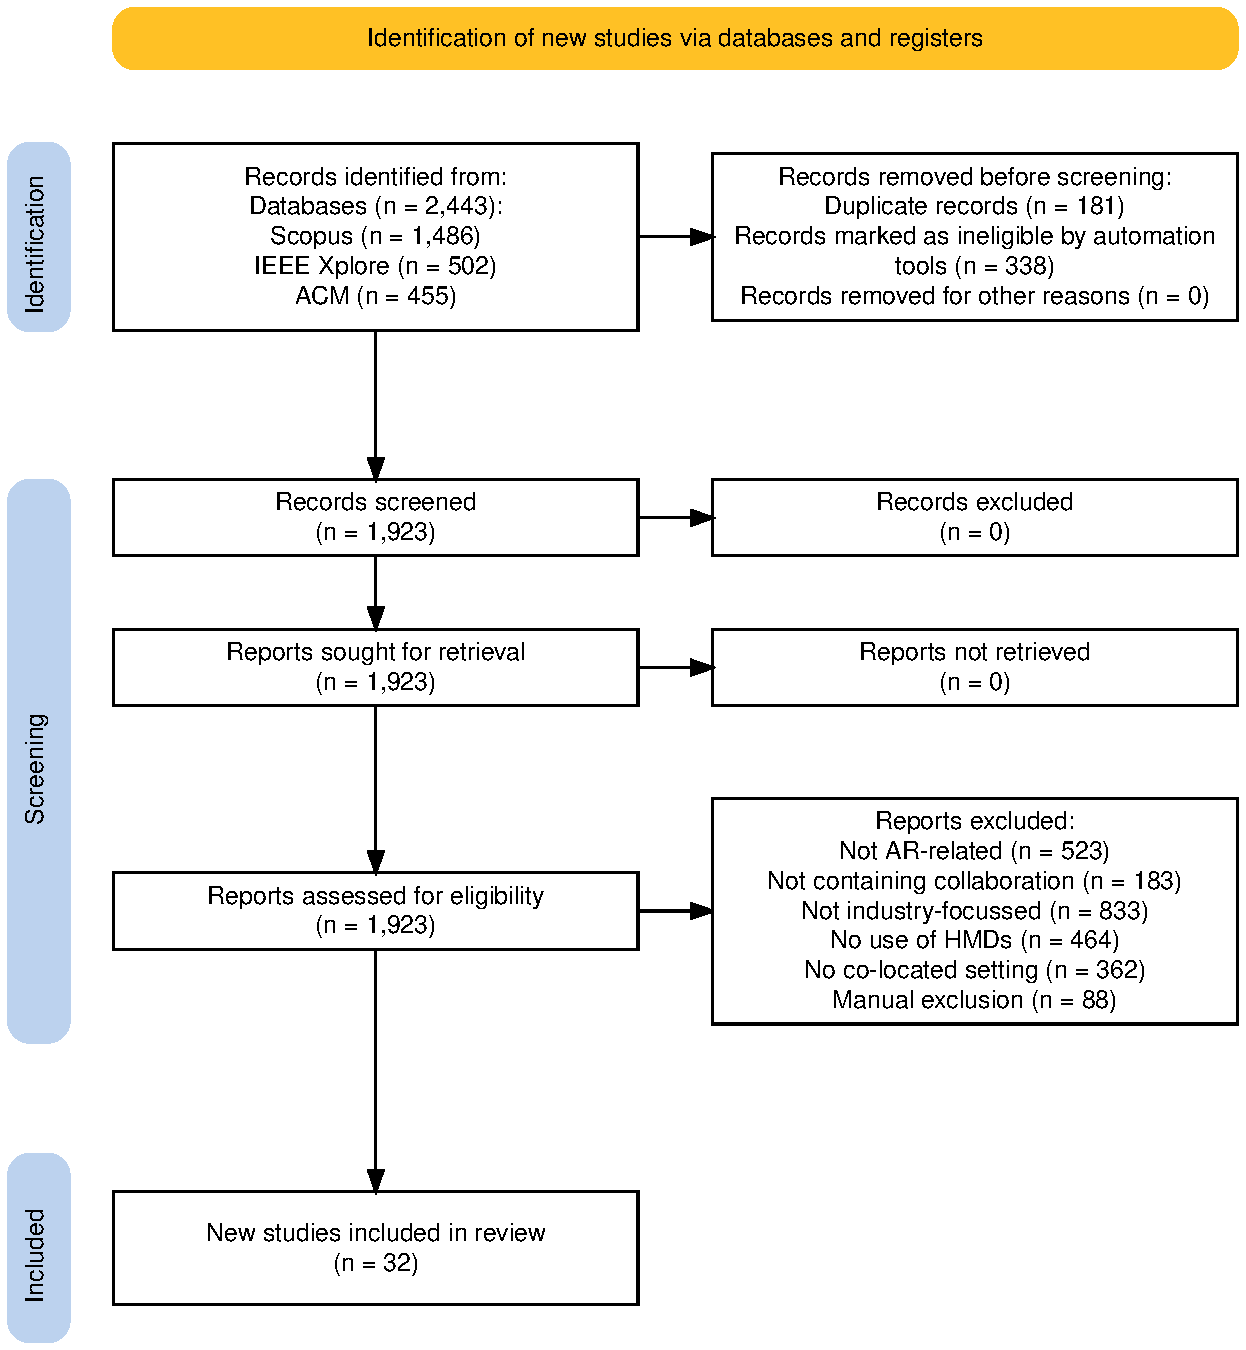
\includegraphics[width=0.8\textwidth]{assets/03/prisma.pdf}
    \caption{PRISMA 2020 flowchart depicting the systematic literature review process. Created using \cite{Haddaway2022PRISMA2020}.}
    \label{fig:prisma-flowchart}
\end{figure}

\section{Results}
\label{sec:lit-results}
\subsection{RQ1:~Types of collaborative AR application in industry}
\label{sec:lit-rq1}

\subsubsection{Archetypes}
An analysis of the 32 primary studies reveals four recurring archetypes for collaborative industrial AR applications. These archetypes are distinguished not just by their application domain but by their goals, dominant interaction metaphors, and the direction of information flow between collaborators.

\emph{Knowledge Transfer and Expert Support} (\textit{n}=12, 37.5\,\%).  
These systems are defined by their primary goal: to mitigate knowledge asymmetry between a remote expert and an on-site operator. The primary UX pattern involves an expert annotating a live video feed of the operator's device. The information flow is characteristically one-to-many, from a single expert to one or more on-site personnel, with only limited communication or interaction between operators. Application scenarios are concentrated in maintenance, repair, and training \cite{aschenbrenner2019comparing,putri2024enhancing}.
The interaction vocabulary is instructional. For example, the system by \cite{wang2022crossPlatform} is designed to allow a remote designer to help an on-site assembler by ``drawing different geometric annotations or creating text labels to help the issue descriptions.'' Evaluation in this archetype is focused on operator performance, with success measured by reductions in task time and error rates, and by managing the operator's cognitive load, making NASA-TLX a relevant, though underused, metric \cite{aschenbrenner2019comparing}.

\emph{Collaborative Creative Workflows} (\textit{n}=8, 25\,\%).  
In contrast to knowledge transfer, these systems focus on co-creation and bridging the design-to-fabrication gap. The primary goal is to empower multiple stakeholders, including non-experts, to participate in the design process through intuitive, direct manipulation of shared digital models. The dominant interaction metaphor is gestural control, often augmented with multimodality (, e.\,g., voice commands) for rapid iteration. \cite{betti2019pop}, for instance, describes a system where ``hand-gestures and speech were used as multimodal interaction with CAD/CAM.'' The information flow is many-to-one and synchronous, with multiple users' inputs converging on a single, shared 3D model. This archetype may blur the line between design and production, as seen in the system by \cite{buyruk2022interactive} where users can ``change the design and fabrication parameters while robotic fabrication continues'', receiving instant visual feedback. Success is measured not only by final output, but by the fluency and speed of the creative process itself, with studies reporting gains in design-decision speed and ideation fluency\cite{buyruk2022interactive,mourtzis2021collaborative}.

\emph{Precision Task Execution in High-Stakes Environments} (\textit{n}=11, 34.4\,\%).  
This archetype is focused on orchestrating human-human and human-robot teams to enhance safety and precision. The UX is defined by procedural guidance; the system leads the user through a sequence of tasks. \cite{deFranco2019intuitive}, for instance, used simple coloured lights as an ``effective non-verbal communication mode to help humans understand the robot's status and actions.'' The information flow is primarily system-to-human. The interaction metaphors are often based on a ``gaze-and-commit'' model, where the user confirms the completion of each step to advance the sequence. For human-robot collaboration, this includes visualising robot intent and safety zones. The work of \cite{cogurcu2023comparative}, for example, evaluated different AR visualisations for robot safety zones and found that virtual ``cage bars'' were preferred because they ``increased the perception of depth and made the safety volume clearer.'' Given the focus on performance and safety, evaluations in this category are dominated by quantitative metrics, with task-time reduction and error-rate being the most frequently reported (Table \ref{tab:evaluation-metrics}).

\emph{Dynamic Problem-Solving in Real-Time} (\textit{n}=2, 6.3\,\%).  
This archetype leverages modern industrial tools like Digital Twins to address unplanned, emergent challenges in real-time. The interaction is not with a static model but with a live, data-rich virtual replica of the physical system. The goal is to enhance system-level resilience and adaptability. The information flow is fully bi-directional and holistic. For example, the HCAS system by \cite{liu2022humanCentric} features a digital twin of the operator that models fatigue and skill level, allowing the system to perform ``adaptive assembly task assignment with operator-centric'' logic. This moves beyond simple guidance to a state of co-active, adaptive collaboration between the human and the cyber-physical system. Evaluation of such systems shifts from operator performance to overall system performance, measuring success by the ability to ``reduce the dependence on human experience and debases the frequency of rework'' \cite{liu2022humanCentric}.


\subsubsection{Evaluations}
\label{sec:lit-evaluations}

The evaluation approaches across the 32 studies reveal a predominant focus on performance and satisfaction metrics. As shown in Table~\ref{tab:evaluation-metrics}, user satisfaction scales were the most frequently reported measure, followed closely by task-time or cycle-time reduction. Safety-related indicators and error-rate measures each appeared in approximately one-third of studies, reflecting the high-stakes industrial contexts. Usability assessments using standardised scales like the System Usability Scale (SUS) were employed in roughly one-fifth of studies, while situational awareness measures appeared less frequently. Notably, only two papers incorporated cognitive load assessments such as NASA-TLX (\cite{aschenbrenner2019comparing} and \cite{chan2022design}), and just one study examined trust in automation (\cite{cogurcu2023comparative}).

\begin{table}[t!]
\centering
\caption{Evaluation metrics reported across the 32 reviewed studies}
\label{tab:evaluation-metrics}
\begin{tabular}{@{}lcc@{}}
\toprule
\textbf{Metric reported} & \textbf{n} & \textbf{\%} \\
\midrule
Task-time / cycle-time reduction & 19 & 59.4\,\% \\
User-satisfaction scales & 18 & 56.3\,\% \\
Error-rate or accuracy & 10 & 31.3\,\% \\
Safety-related indicators & 9 & 28.1\,\% \\
Usability (, e.\,g., SUS) & 6 & 18.8\,\% \\
Situational awareness & 6 & 18.8\,\% \\
Cognitive load / NASA-TLX & 2 & 6.3\,\% \\
Trust in automation & 1 & 3.1\,\% \\
\bottomrule
\end{tabular}
\end{table}


\subsection{RQ2:~User-experience design approaches in collaborative AR applications in industry}\label{sec:lit-rq2}

Effective User Experience (UX) design is paramount for the successful adoption of collaborative Augmented Reality (AR) applications in industrial settings. Research across various industrial domains, from manufacturing and assembly to maintenance and repair, highlights several key UX design approaches that have been utilised to enhance collaboration, improve efficiency, and increase user satisfaction. The evidence suggests that a human-centred approach, focusing on intuitive interaction, shared context, and clear communication, is crucial for unlocking the full potential of AR in these complex environments.

The reviewed literature reveals four primary UX design approaches that have been consistently employed across collaborative industrial AR applications:

\subsubsection{Shared 3D Spatial Views}

A fundamental principle in collaborative AR is the establishment of a shared visual context, where multiple users can simultaneously view and interact with the same virtual information overlaid onto their physical workspace. This approach features real-size AR projections or holograms shared across multiple users, supporting synchronised annotations and spatially aligned overlays.

Studies consistently demonstrate that shared visual context is critical for successful collaboration. \cite{aschenbrenner2019comparing} found that shared visual context was crucial for collaborative settings and that adding this element to mixed-reality systems leads to superiority in both task and human factor metrics. This finding is echoed in production line planning applications, where co-located workers wearing HMDs share a common visual context on the planned position of robots and production machines \cite{aschenbrenner2018collaborative}.

The advantages of shared 3D spatial views include enhanced spatial and situational awareness, reducing miscommunication between collaborators. Demonstrated improvements in task time and error rates have been reported. Technical and human-factor challenges, including limitations imposed by the field of view (FOV) of HoloLens devices, and high cognitive demands when spatial alignments are imprecise or laggy, present challenges for practical implementation.

\subsubsection{Multimodal Interaction Interfaces}

To make AR systems accessible and efficient, especially for users who may not be tech-savvy, providing multiple and natural interaction methods has become a widely adopted approach. This includes combining gesture, voice, and touch inputs for user control, often supported by visual icons and AR overlays.

This approach lowers the barrier to entry for using complex AR systems. \cite{betti2019pop} found that with a multimodal interface using hand gestures and speech, non-professionals could easily follow visual cues in AR and utilize their existing communication skills to control 3D modelling and robotic fabrication with minimal training time. This demonstrates that intuitive interaction methods can make sophisticated technology accessible to a broader audience. \cite{gemito2023mixed} similarly highlights the use of holographic hardware devices that respond to users' gaze, gestures, and voice commands.

The advantages include providing redundancy in input modes, ensuring usability even in noisy or high-distraction environments, while reducing physical strain and increasing engagement through naturalistic interactions. However, gesture and voice recognition systems are prone to errors, especially in complex industrial settings, and over-reliance on multimodal input may overwhelm less experienced users.

\subsubsection{In-Situ and Context-Aware Information Display}

A core strength of AR is its ability to deliver information precisely when and where it is needed. This approach involves overlaying digital instructions, safety warnings, and performance data directly onto the physical work environment, essentially providing sequential collaboration where tasks are divided into individual, sequential steps with AR providing guidance at each stage.

This approach has been shown to significantly improve situational awareness, safety, and task performance. \cite{putri2024enhancing} found that greater situational awareness and real-time visual signals lead to considerable increases in incident prevention through the use of AR headsets that deliver real-time safety advice, visual cues, and training simulations. Furthermore, \cite{cogurcu2023comparative} reported that virtual cage bars were preferred by users for a real robot arm because they increased the perception of depth and made the safety volume clearer.

The advantages include ease of understanding and engagement with minimal training, making it well-suited for structured tasks such as step-by-step assembly or design reviews. However, this approach may lack real-time interaction between users and can lead to reduced collaboration fluidity in highly dynamic or creative workflows.

\subsubsection{Role-Based Interfaces and Information Filtering}

In collaborative industrial settings, different users often have distinct roles and responsibilities. Effective UX design accounts for this by providing role-based interfaces that filter and present information relevant to each user's specific tasks, thus avoiding cognitive overload. This approach often incorporates direct holographic feedback for real-time adjustments in co-located environments.

\cite{wang2022multiPerson} proposed a role-based collaborative method for a multi-person AR assembly evaluation system, where users could assume the roles of operator or evaluator, each with different system authorities and access to information. This approach allows for a more focused and efficient collaborative workflow. The need for such tailored interfaces is further supported by \cite{yang2023usability}, where users in a robot control role expressed a need for different information such as trajectory, target, and digital twins compared to those performing manual fabrication tasks.

The advantages include high levels of engagement and user satisfaction due to intuitive interaction, and effectiveness in tasks requiring high precision, such as collaborative manufacturing. However, this approach demands frequent calibration to ensure spatial alignment and has limited scalability for large teams due to device or environment constraints.

\subsubsection{Evidence of Enhanced Collaboration and User Satisfaction}

The application of these UX design approaches has yielded compelling evidence of their effectiveness in industrial settings, backed by both quantitative and qualitative data. \cite{gemito2023mixed} reported a 30\% reduction in total assembly time and a 50\% reduction in learning time for new operators using a mixed reality guidance system. 

In terms of user satisfaction, \cite{yang2023usability} reported a mean System Usability Scale (SUS) score of 73.5 for a collaborative AR system for timber fabrication, which is considered above average. The feedback was overwhelmingly positive, with participants expressing feelings of safety when they could see and predict their collaborators' movements. Participants also indicated high confidence and ease of use, with a majority agreeing that most people would learn to use the system very quickly.

Quantitative improvements have also been demonstrated in task accuracy. \cite{deFranco2019intuitive} found that an AR interface for providing force feedback resulted in a statistically significant improvement (p-value < 0.01) in task accuracy compared to a standard monitor-based feedback system during a collaborative polishing task.


\subsection{RQ3:~Technical challenges in collaborative AR applications in industry}
\label{sec:lit-rq3}

\subsubsection{Implementation ecosystem}

Four-in-five systems rely on Microsoft's optical see-through head-mounted displays (HoloLens~1 or~2).  This homogeneity simplifies cross-study comparison, but it also limits ecological validity for vendors whose devices differ in optics, field-of-view, or tracking stack.  On the software side (Table~\ref{tab:rq3-software}) Unity plus MRTK is the dominant rendering pipeline, often bridged to ROS/MoveIt when robots are involved.

\begin{table}[t!]
\centering
\caption{Most-used hardware platforms across the 32 studies}
\label{tab:rq3-hardware}
\begin{tabular}{@{}lcc@{}}
\toprule
\textbf{Hardware category} & \textbf{\# papers} & \textbf{\%} \\ \midrule
Microsoft HoloLens (1st gen)            & 14 & 43.8\,\% \\
Microsoft HoloLens 2                    & 13 & 40.6\,\% \\
Industrial robot (any make)             &  8 & 25\,\% \\
Tablets (worker sidekick / expert view) &  4 & 12.5\,\% \\
Desktop / VR terminal (aux display)     &  3 & 9.4\,\% \\
Projection-based SAR                    &  2 &  6.3\,\% \\
Smartphone / mobile AR                  &  2 &  6.3\,\% \\
Wearable sensors (IMU, EMG, etc.)       &  2 &  6.3\,\% \\
HTC Vive (VR context switch)            &  1 &  3.1\,\% \\
Azure Kinect depth camera (aux tracking)&  1 &  3.1\,\% \\ \bottomrule
\end{tabular}
\end{table}

\begin{table}[t!]
\centering
\caption{Dominant software / toolchains}
\label{tab:rq3-software}
\begin{tabular}{@{}lcc@{}}
\toprule
\textbf{Software / framework} & \textbf{\# papers} & \textbf{\%} \\ \midrule
Unity engine (C\#,\;MRTK, URP) & 14 & 43.8\,\% \\
ROS / MoveIt (robot middleware) &  10 & 31.3\,\% \\
Custom in-house pipelines       &  3 &  9.4\,\% \\
Grasshopper (+ Rhino 3D)        &  3 &  9.4\,\% \\
MRTK (named explicitly)         &  4 &  12.5\,\% \\
Metaio (legacy Android SDK)     &  1 &  3.1\,\% \\
Vuforia (marker tracking)       &  1 &  3.1\,\% \\ \bottomrule
\end{tabular}
\end{table}


\subsubsection{Technical Challenge Categories}

The technical challenges reported across the reviewed studies can be organised into four primary categories: hardware constraints, spatial anchoring and tracking, network communication, and system performance.

\paragraph{Hardware Constraints}

Hardware limitations represent the most frequently reported challenges, with ergonomic and display constraints being particularly problematic. \cite{cogurcu2023comparative} specifically notes that the HoloLens 1 is ``uncomfortable to wear for prolonged periods'' and identifies limited field of view as a major issue. While \cite{yang2023usability} reports that the HoloLens 2 offers improved comfort for extended wear, usability concerns persist, with one participant noting: ``in the beginning OK but I got [a] headache after 45 minutes.''

Tracking accuracy represents another significant hardware constraint. \cite{aschenbrenner2019comparing} highlights issues with comparing across different hardware modalities and confirms that camera resolution directly affects tracking accuracy. Computational limitations also emerge as bottlenecks, with \cite{stacchio2023annHoloTator} requiring remote server computation for the majority of processing tasks, while \cite{schmidt2022augmentedReality} reports performance issues affecting both CPU and GPU utilisation.

\paragraph{Spatial Anchoring and Tracking}

Multi-user spatial anchoring emerges as a persistent technical challenge across the reviewed studies. While SLAM works adequately for single users, \cite{martins2024multiUser} identifies significant issues in dynamic environments with multiple participants. The challenge becomes more complex when users need to share a common spatial reference frame for effective collaboration.

Only six studies (18.8\,\%) employ explicit marker-based tracking systems (, e.\,g., ArUco markers or Vuforia), with just one study reporting a fully marker-less SLAM pipeline. The remaining 25 studies rely primarily on the headset's internal spatial anchor-based tracking, which may partially explain why drift and misalignment emerge as common issues across these implementations.

\paragraph{Network Communication}

Network-related challenges prove complex, even with sophisticated custom networking protocols. \cite{vidalBalea2020creating} and \cite{wang2022crossPlatform} both implement custom networking solutions targeting sub-10ms network delays, yet still encounter significant issues. Despite this technical sophistication, \cite{vidalBalea2020creating} reports problems with packet loss when scaling to multiple concurrent users, though 5G connectivity provides some improvement. Communication latency appears to be a more critical factor than bandwidth requirements\cite{wang2022crossPlatform}.

\paragraph{System Performance and Scalability}

Performance optimisation represents an ongoing challenge, particularly when scaling collaborative AR systems. Multiple studies report the need for computational offloading to maintain acceptable frame rates and interaction responsiveness\cite{stacchio2023annHoloTator,schmidt2022augmentedReality,gemito2023mixed}. The complexity increases significantly when integrating with existing industrial systems, as evidenced by the prevalence of ROS/MoveIt middleware in robot-integrated applications.

\subsubsection{Reported Solutions and Mitigation Strategies}

The literature reveals several recurring mitigation strategies organised by challenge category:

\paragraph{Hardware Constraint Mitigations}

Solutions for addressing hard technical limitations like field-of-view remain limited. \cite{aschenbrenner2018collaborative} implemented ``miniature god-view overviews'' that provide complete scene context when the primary display clips large objects, while \cite{schmidt2022augmentedReality} rotates and scales UI elements to the user's point of view.

For ergonomic constraints, studies recommend structuring work cycles to accommodate device limitations rather than attempting to extend wearing times. If available, backup devices can be hot-swapped to prevent downtime due to battery life or overheating\cite{yang2023usability}.

\paragraph{Spatial Tracking Solutions}

Multiple approaches address the spatial tracking challenge. \cite{martins2024multiUser} implements fiducial markers to establish common reference frames across multiple devices. \cite{aschenbrenner2018collaborative} provides minimap-based ``god-views'' for manual realignment when automatic registration fails.  Manual recalibration prompts, implemented by \cite{chan2022design}, help maintain tracking accuracy over extended sessions. More sophisticated solutions include the digital twin overlays employed by \cite{buyruk2022interactive}, which provide live feedback during fabrication to maintain spatial consistency.

\paragraph{Network Communication Solutions}

Network challenges are addressed through multiple two complementary strategies. On the one hand, custom networking protocols like those implemented by \cite{vidalBalea2020creating} and \cite{wang2022crossPlatform} prioritise low-latency state synchronisation over high-bandwidth media streaming. Message queuing schemes that prioritise low-payload state differences over high-payload media content (like MQTT employed by \cite{schmidt2022augmentedReality}) are increasingly common. On the other hand, edge computing deployments help reduce round-trip latencies by processing computationally intensive tasks closer to the end users.

\paragraph{Performance Optimisation Strategies}

Computational offloading strategies include cloud-based processing for computer vision workloads and distributed rendering architectures (, e.\,g., falling back to holographic remoting like \cite{stacchio2023annHoloTator}). In the majority of cases, the authors appear to have simply scaled back their ambition to achieve acceptable frame rates and interaction responsiveness. For example, \cite{reis2021caseStudy} reports that ``[d]ue to the hardware limitations, it was not possible to load larger models and run them simultaneously''.


% Takeaway: 
% Specific UX decisions always grounded in task design
% It seems like there's a lot of "fine tuning" in interaction design for the specific "course"

% --------------
% Misc:
% Ideally I already ground task design here (Bridge Building is cool because xyz)
% There is this TUM(?) course that does it, so I _could_ reference that (outside the literature), but grounding would be useful
